\chapter{Results}
\label{chapter:Chapter 5}
\lhead{Chapter 5. \emph{Results}}

In this Chapter, we present a group of experiments on the MAD-F capabilities. Firstly, we undertake data ingestion and storage performance test, which is followed by a exploratory analysis of the gathered data. Secondly we validate each of the ADS modules, starting with the RB-ADS Experiment, where the data that was collected previously is Experiment is injected in this module with the help of a simulator. After an Experiment over the ADS is conducted, where for each of the anomalies that are detected we provide and exploratory analysis of the results.
The \emph{validation} of the results presented in this Chapter, can only truly be done by Maritime Officer.The what is to be called as reported anomalies in this work must not be interpreted as an actual maritime illegality, but only as a possible anomaly, which needs always to be validated by Maritime Officer.


\section{Data Ingestion Experiment}
\label{section: Experiment Data}
Data Ingestion Experiment refers to the Experiment were we accessed the performance of the Data-Ingestion capability of MAD-F. In order to achieve this, we provided a real NMEA feed as input to our the Data Ingestion Module. This NMEA feed was provided by the Portuguese Navy via the \textsc{Marisa} project, and it was a feed that aggregated messages from multiple antennas around Portugal.
 
With the provided feed, we allowed the Framework to be executed for five straight days, thus ingesting pre-processing and wrangling the NMEA feed into Behavioural Points. As for this experiment we used a real NMEA feed, the messages were firstly decoded into a readable format, and only then after the whole pre-processing was done, the $BPs$ were stored in the Trajectory Extraction Cassandra Data-Base.

From the 5 days of data acquiring, we acquired from a total of $2,259,615$ $BPs$ from $5563$ different Vessels.
As the provided feed did not broadcast any vessel static information, from the vessel that generated each message. The vessel static information namely the vessel type and country of origin, were scrapped from the internet using the developed \emph{Vessel Type Scrapper} which we presented in~\ref{subsection: Vessel Type}. 
From the $5563$ Vessels $6$ of them were not considered for this Experiment. The MMSI of this vessels was either not found or their MMSI was representative for more than one Vessel. The latter, represents an abnormal situation which could be denominated Spoofing, as represented by the authors in~\cite{Ray2015DeAISRisks} or in \footnote{http://globalfishingwatch.org/data/spoofing-one-identity-shared-by-multiple-vessels}. This is a occurring problem when handling AIS data, and will be discussed in the future work.
In Figure~\ref{fig: 5 Vessel Type Distribution}, we present the vessel type distribution from the acquired $BPs$.
\begin{figure}[H]
	\centering
	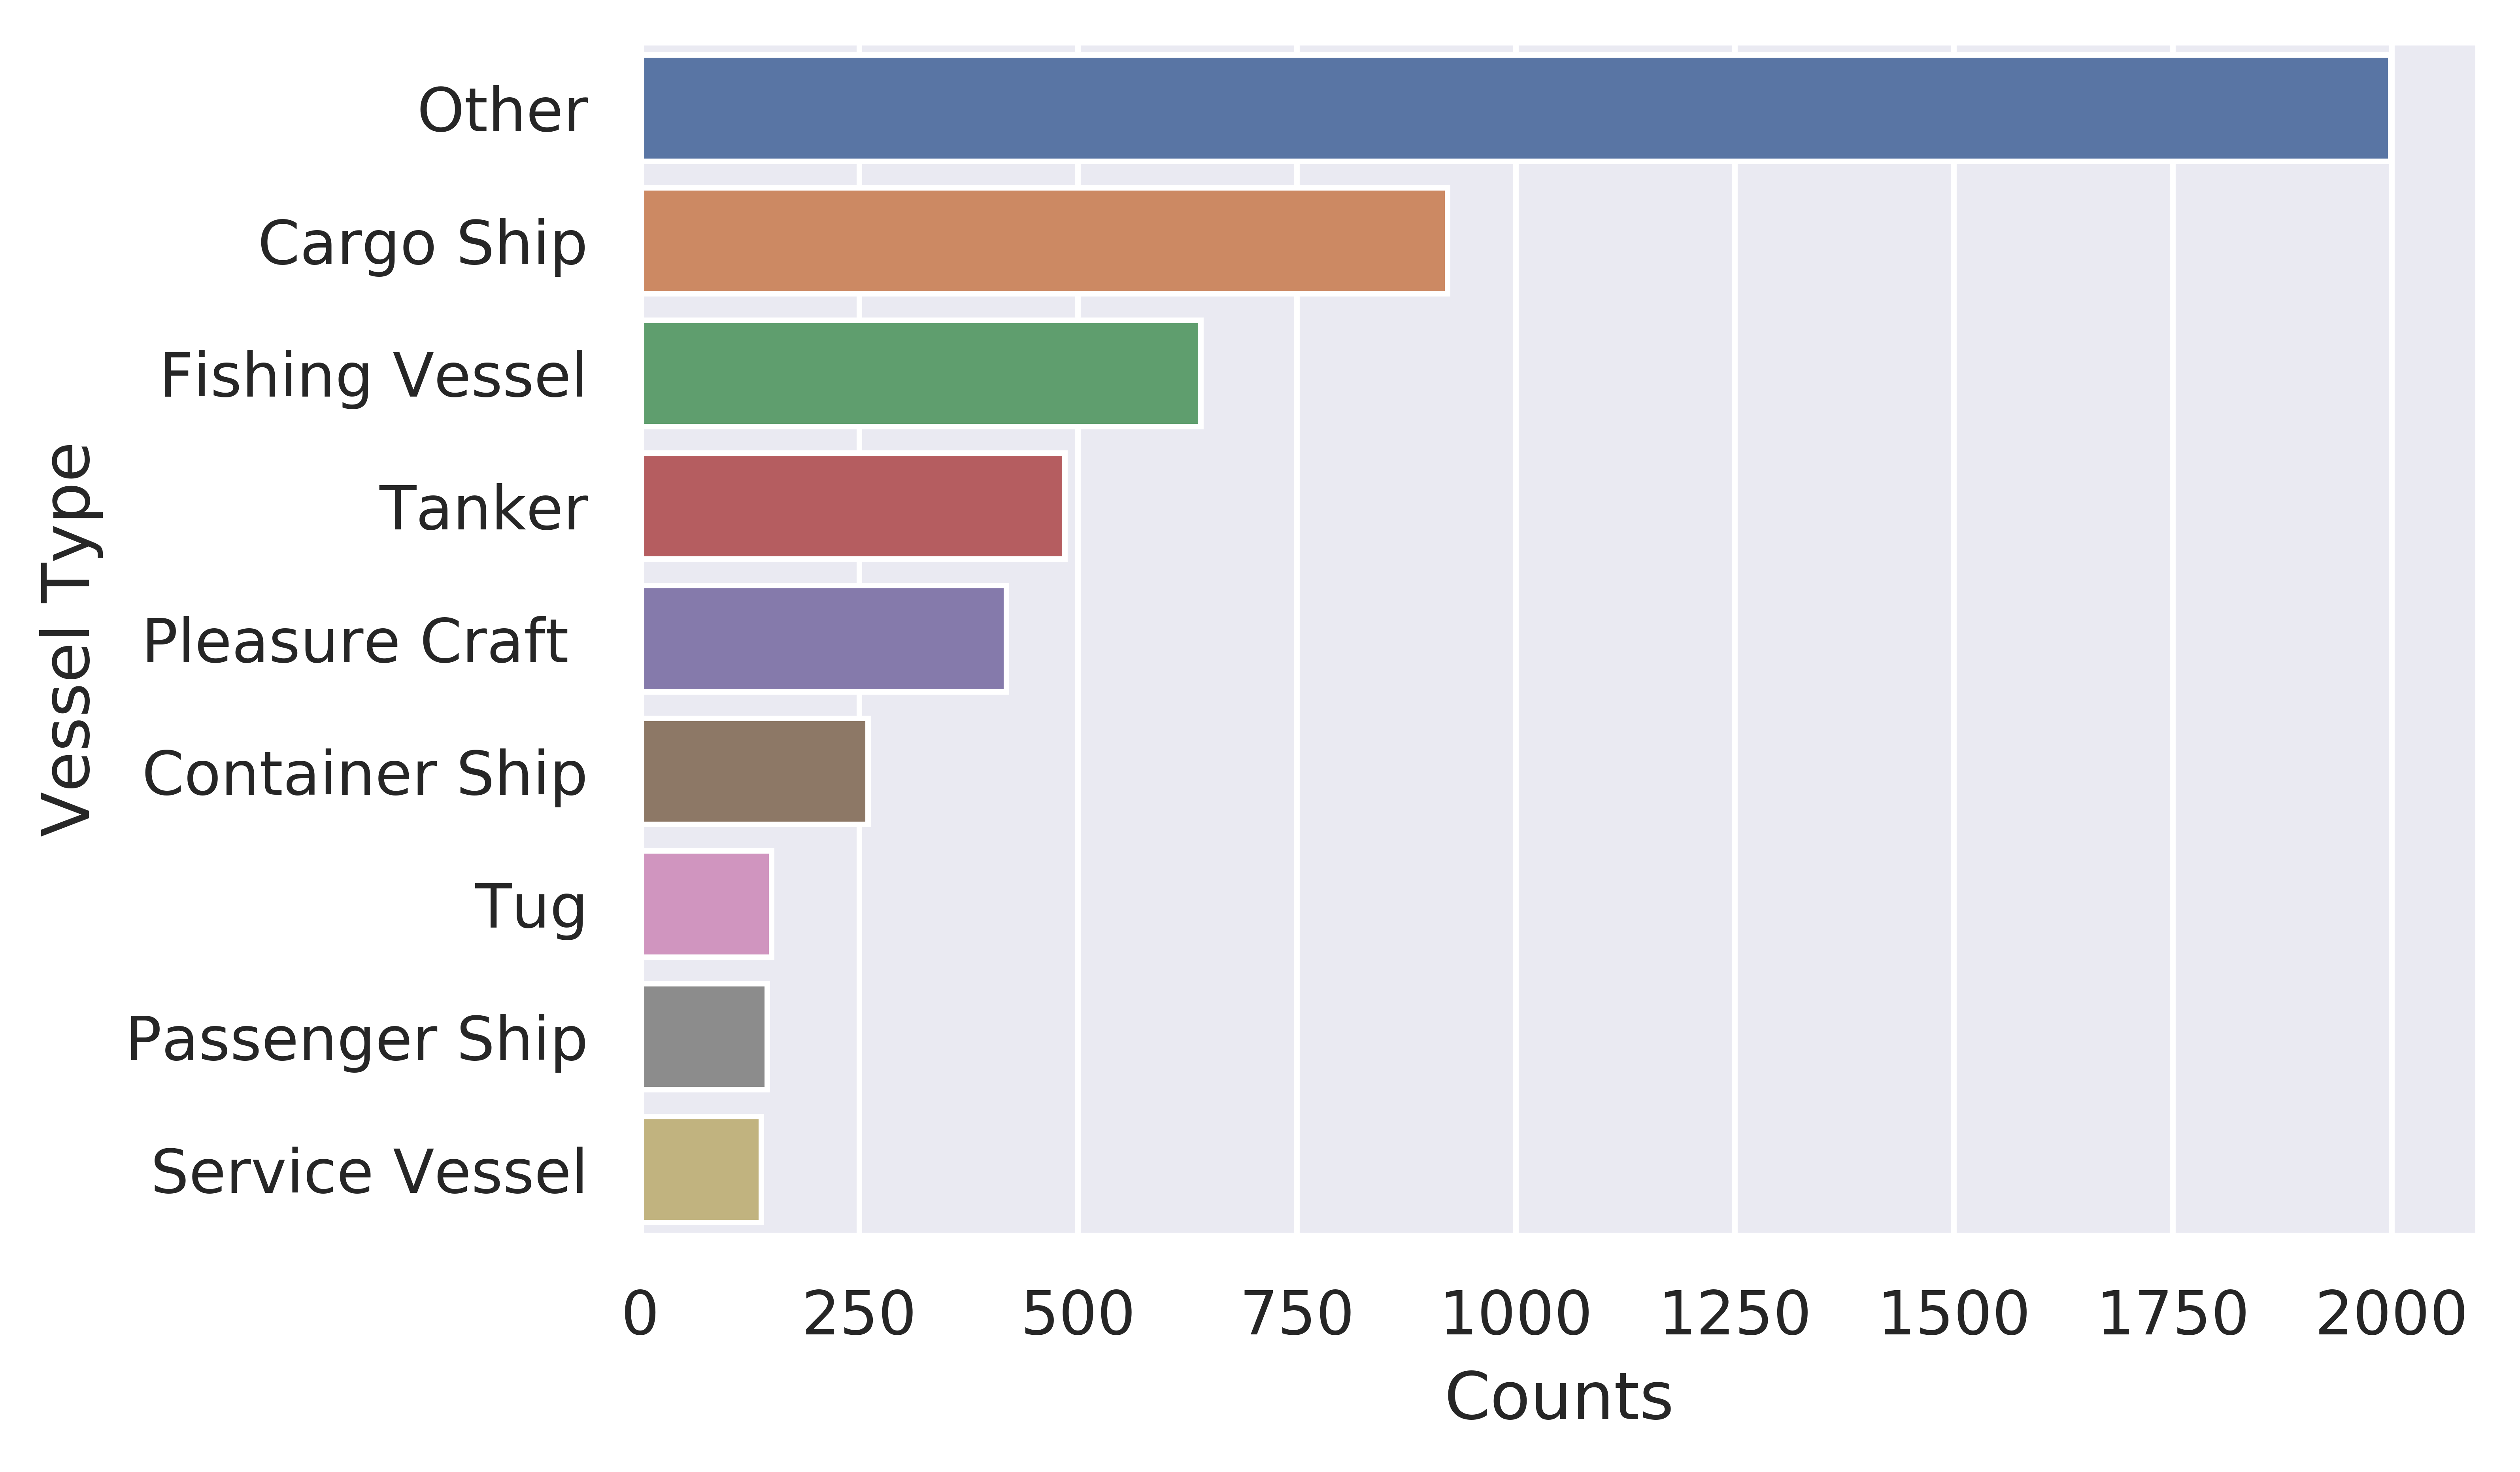
\includegraphics[scale = .7]{figures/Ch5/DataValidationVesselType.png}
    \caption{Vessel Type distribution of $5157$ Vessels.}
    \label{fig: 5 Vessel Type Distribution}
\end{figure}

Another feature calculated while transforming data into $BPs$ was the point-based closest distance to coast and ports, which was done to every received NMEA AIS message received. In order to validate if this calculation were in fact being accurate, we analised based on the received $BPs$ which countries were the closest and the respective ports.
In Table~\ref{Table: 5 Closest Countries} we present the distribution of closest countries. 
\begin{table}[H]
\centering
\caption{Most Frequent Closest Countries Counts.}
\label{Table: 5 Closest Countries}
\begin{tabular}{@{}lcc@{}}
\toprule
Country & Counts & Counts(\%) \\ \midrule
Spain & 1,306,436 & 58\% \\
Portugal & 663,841 & 29\% \\
Morocco & 259,776 & 11\% \\
Gibraltar & 26,885 & 1\% \\
France & 2,516 & 0.1\% \\
Cabo Verde & 161 & 0.007\% \\ \bottomrule
\end{tabular}
\end{table}
In Table ~\ref{Table: 5 Closest Ports} we present a post validation of the closest Ports for every received message. This was done as a way to validate if whether the closest Ports seems plausible, as a single message validate would be impossible. Thus, from tin Table XX we present the subset of top most frequent closest ports from the $69$ total possible Ports, which are plotted in Orange in figure XX.
\begin{table}[H]
\centering
\caption{Most Frequent Closest Ports Counts.}
\label{Table: 5 Closest Ports}
\begin{tabular}{@{}lcc@{}}
\toprule
Port Name & Counts & Counts(\%) \\ \midrule
Lisboa & 142,464 & 6,3\% \\
Villa Garcia De Arosa & 112,254 & 5\% \\
Europa Point(Gibraltar) & 109,273 & 4,8\% \\
Lagos & 107358 & 4,7\% \\
Las Palmas & 106,116 & 3,5\% \\
Cadiz & 79,577 & 3,5\% \\
La Corunha & 78,929 & 3,5\% \\
Malaga & 65,227 & 2,9\% \\
Vigo & 64,759 & 2,9\% \\
Faro & 62,925 & 2,9\% \\ \bottomrule
\end{tabular}
\end{table}

We further validated the reception, by displaying all the 2.2 $BPs$ into a density plot. As scattering Millions of points is computational heavy, and if "normal" plotting packages were to be used,  not possible with the Hardware specifications presented in XX. Thus the density plots presented in this Chapter were using the\footnote{http://vaex.astro.rug.nl}, which is optimised huge data-sets. 

\begin{figure}[H]
	\centering
	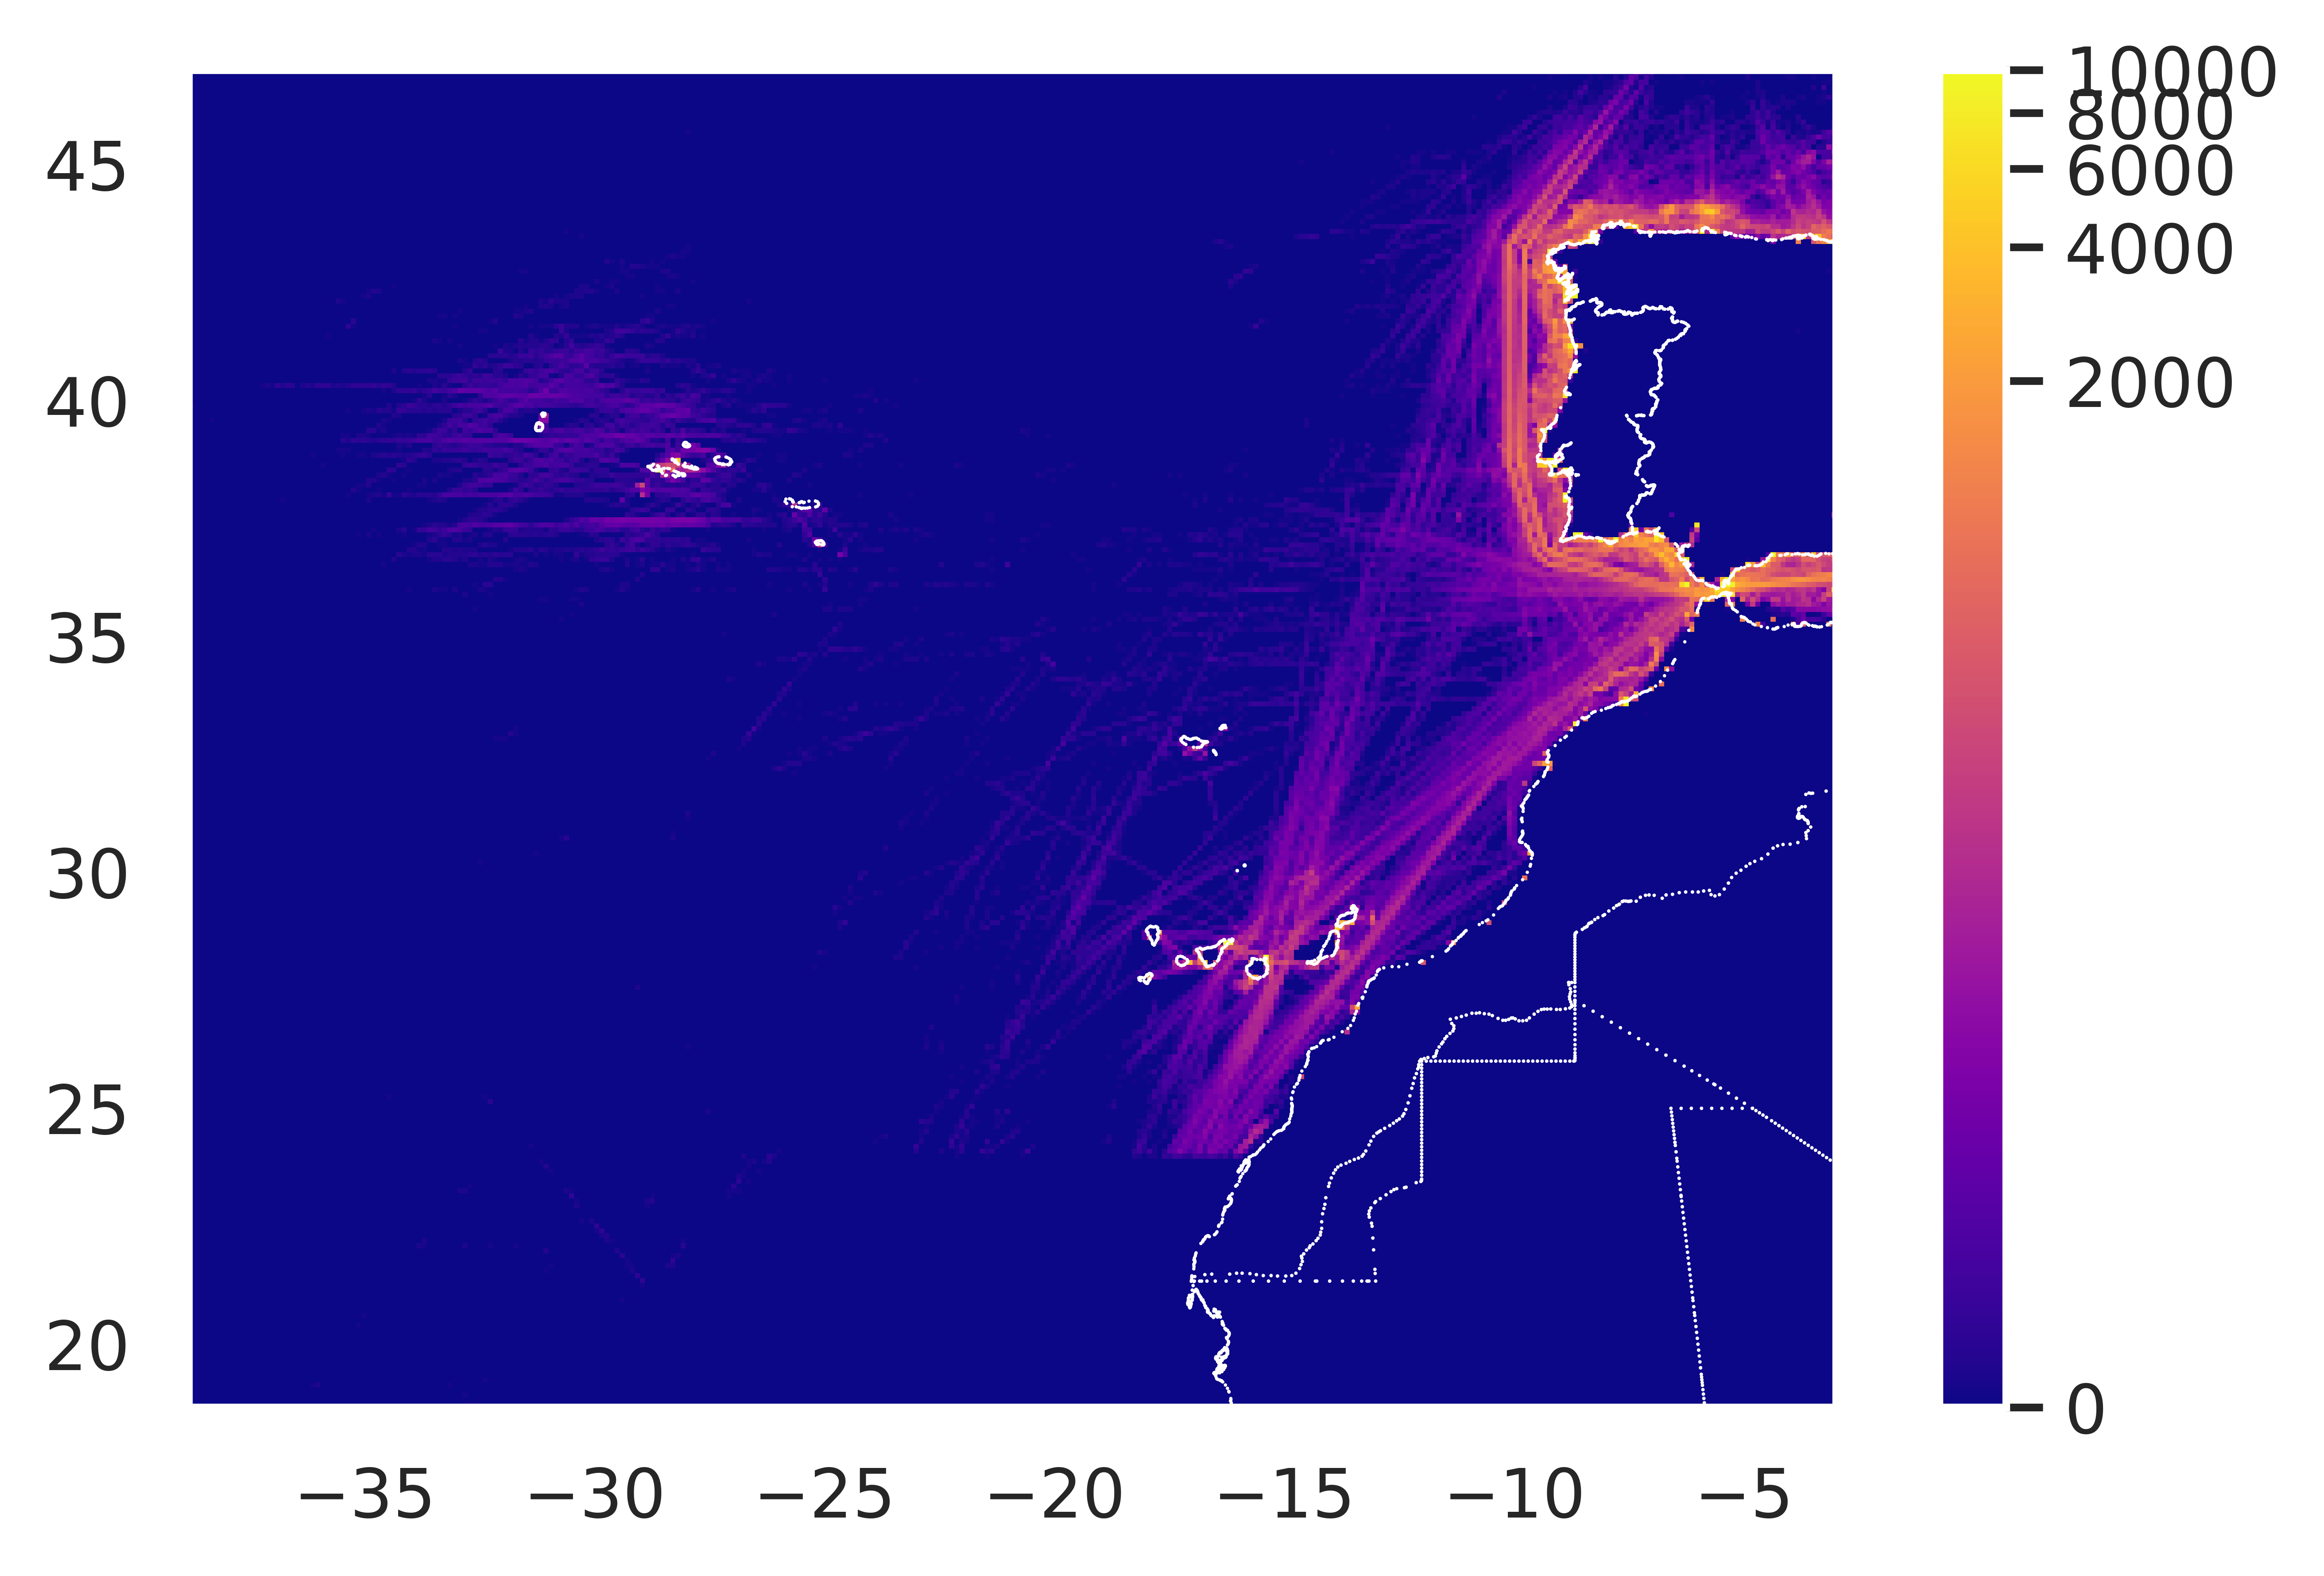
\includegraphics[scale = 1]{figures/Ch5/ThesisExpDensity.png}
    \caption{Density map, with all the aprox. $2.2$ Milion points.}
    \label{fig: 5 Exp1DensityMap}
\end{figure}

What we found by analysing Figure~\ref{fig: 5 Exp1DensityMap} is that in fact the messages that were received via the Portuguese Navy antennas. Which explains the reception of messages near the Madeira and Azores islands.  What is possible also to analyse in the Figure, is nearby the Portuguese coastal line a few lines of high density traffic show up. These lines represent the navigational lanes, and when navigation in this lanes vessels tend to have a more standardised behaviour. Such fact can be explored other types of AD, and is presented by the authors in~\cite{Yan2016} and~\cite{Silveira2013UsePortugal}. The aknoledege of this lanes for anomaly detection will be endorsed in future work.


\section{Rule Based Anomaly Detection Service Experiment}
\label{section: RB-ADS Experiment}

This experiment was conducted, to validate the real time capabilities of the Rule Based Anomaly Detection Service Module. In order to validate such capabilities of this module, we focused this experiment on the validation by analysis of the anomalies generated by this module, and whether this module could function in near-real time or not.

To tackle this problem, we injected the resulting $BPs$ from the Experiment \ref{section: Experiment Data} in the RB-ADS module. Therefore this experiment was not conducted using the real-time data NMEA feeds. If the feed would be used,  we would loose control of the incoming data, which would make this experiment not possible to replicate.

As the results from the Experiment~\ref{section: Experiment Data} were stored in the trajectory data-base, they could be accessed multiple times. We thus developed a $BPs$ simulator which from the stored trajectories would simulate the real reception of AIS streams (from the perspective of the RB-ADS module).

The simulator, thus gathers $BPs$ from the trajectories (or a group of) stored in the trajectory data-base, and send this $BPs$ to the RB-ADS, as presented in \ref{fig: 5 BPs Simulator}.

\begin{figure}[H]
	\centering
	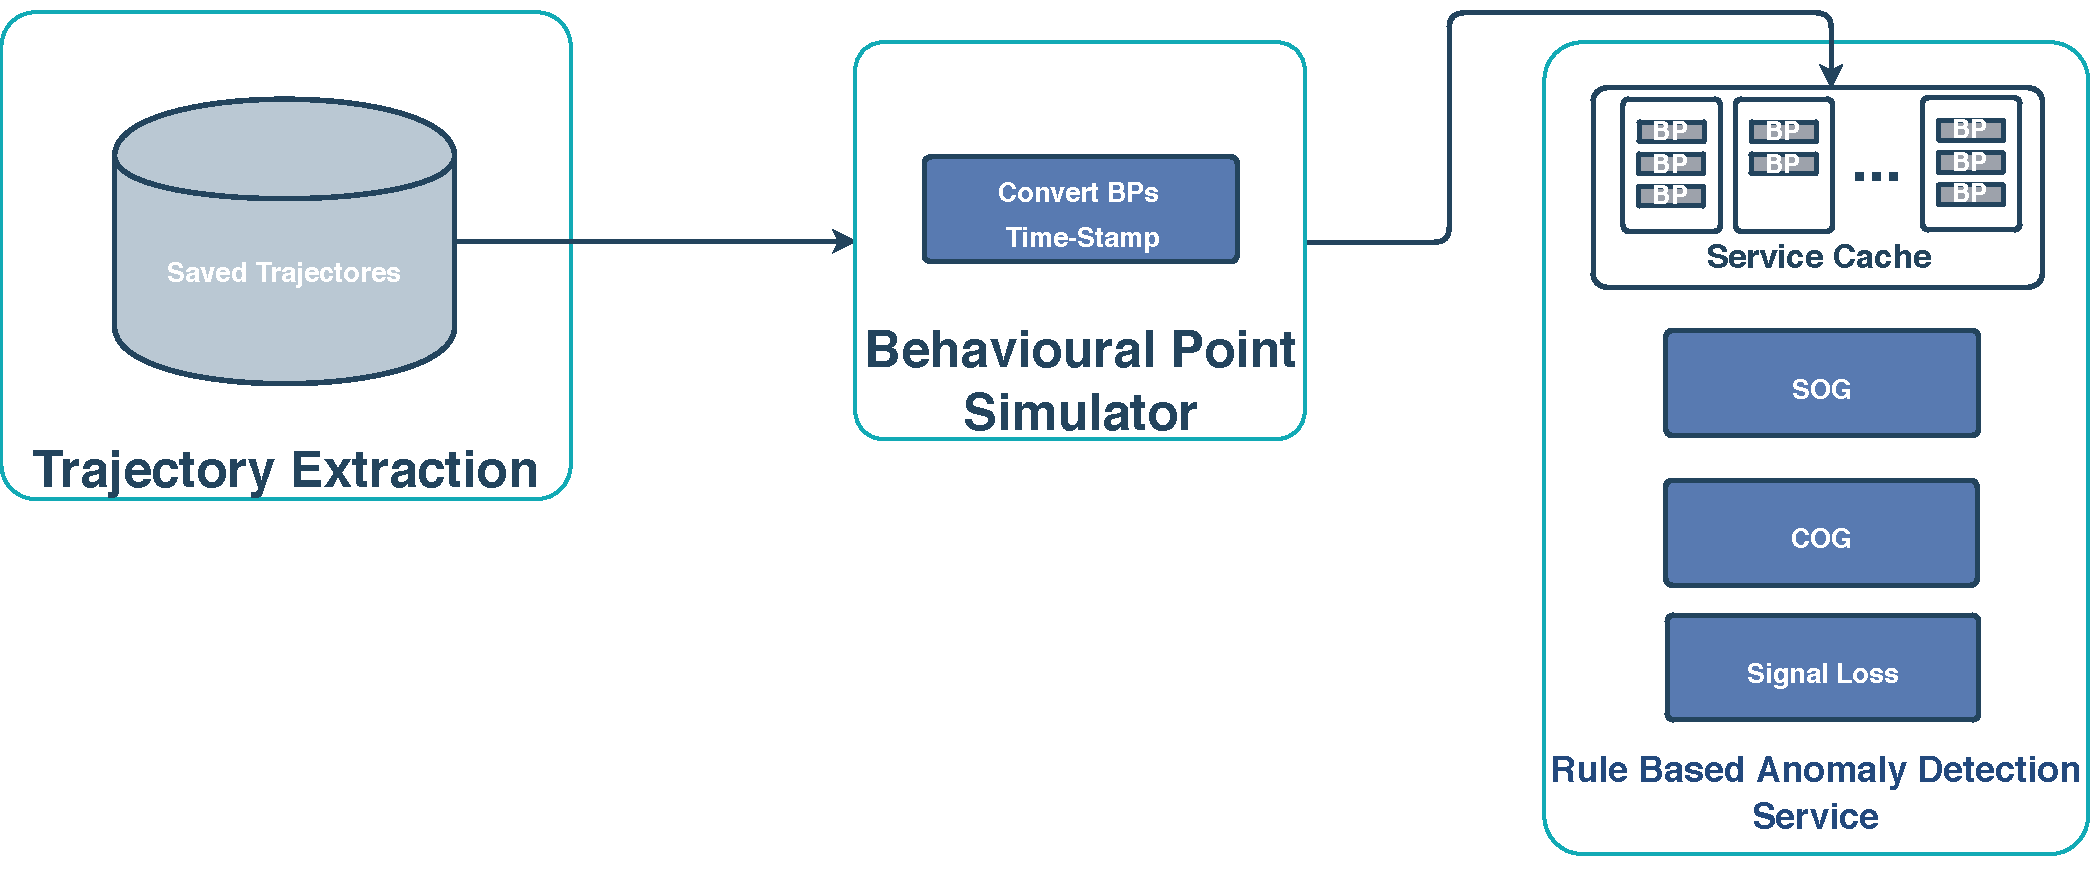
\includegraphics[scale = .3]{figures/Ch5/SRM-Exp-Simulator.pdf}
    \caption{BPs Simulator.}
    \label{fig: 5 BPs Simulator}
\end{figure}

The simulator worked by setting the a \textbf{Initial-Simulated-Time} as if it was the current Time. And based on this \textbf{Initial-Simulated-Time}, the following $BPs$ would be sent with a 
For this Experiment the \textbf{Initial-Simulated-Time} was set first received $BP$ from the Experiment \ref{section: Experiment Data}, which was XXXXXXTODOXXXXXX.  

As it would be not practical waiting 5 days for this Experiment, we 

Thus, we ran RB-ADS with the simulator setted to a speed of X, and with the RB-ADS parameters represented in table XX.

\missingfigure[]{Table RB-ADS paramenters XX}

With the parameters described above, we found XX anomalies and ALALALAL AAHAHH AJAJAJ need to do the simulation

\section{Anomaly Detection Service Experiment}
\emph{ADS Experiment} was for this work, our validation method of the AD functionalities developed in this module. The steps towards this experiment were similar to the Experiment~\ref{section: Rule Based Anomaly Detection Experiment}. Although, as the motive for the development of this module was to access more complex anomaly detection which would use huge batches of data, we did not conduct this experiment with the data stored which was pre-processed in ~\ref{section: Experiment Data}, for the RB-ADS Experiment(\ref{section: RB-ADS Experiment}).
This experiment was then conducted with the same data-set which was used in our initial data-analysis(Section\ref{section: Data Analysis}). We chosen to use this data-set, as it in fact represented an huge batch of data. 

Before performing of the \emph{ADS Experiment} itself, the raw data-set was injected in the MAD-F as a single batch of data. This transformed a the AIS data-set into a normalised set of $BPs$, which was kept stored in \emph{Trajectory Data-Base}. What is to note is that if this group of $BPs$ were to be stored as files, these files would be nearly 3 Gigabytes (if stored as .csv type files).
As the transformation of the data-set in $BPs$ made the data-set pass through the "pre-processement" pipeline. This cleaned the whole data-set which was of initially 18,84 Million rows (AIS messages), from 4555 different Vessel, into approximately 17,10 Million $BPs$.
After the $BPs$ were store as trajectories, and additional "manual" filtering was done. We filtered the trajectories with a size inferior of 100 $BPs$. This filtering only slightly reduced the number of total $BPs$ considered for this experiment to 17,06 Million, although the number of considered Vessels was dramatically reduced to 1588 Vessels.

The ADS experiment was divided into two Sections. The first section presents the results obtained for the Vessel Rendezvous detection, and the second section presents the results for the Incoherent Navigational Status and Time Space incompatibility. 

\todo[inline]{ver so como acabar esta intro...}
As the ADS module was developed to detect 3 different types of experiment, but with two of this anomalies bei we divided this whole experiment into t
Thus, we ran the Anomaly Detection Service with the configurations presented under in Table XX, with a Set of   $BPs$ from 4555 different Vessels. 

The ADS presenting 2 different types of anomalies, we divided this experiment in two the Rendezvous detection and the Wrong Status Validation. Thus in the following subsections, we present the results (being the anomalies generated) and the performance of each sub experiment.


\subsection{ADS - Rendezvous Experiment}
\label{subsection: ADS - Rendezvous Experiment}
This subsection, shows the results and our analysis of the results obtained for the Rendezvous Experiment.
We conducted this Experiment on the the the batch of data which was described above. The Rendezvous detection, as any other module was developed to be configured with the set of parameters most adequate for the situation which would be deployed. The choice of parameters in any real scenario would be done by Maritime Experts. Although for the sole porpoise of this experiment, the choice of parameters was done by us. This, in this Experiment we present four different set of configurations(Table~\ref{Table: 5 ADS Rendezvous input paramenters}), and explore the diferences fof the results each set of configurations produces .

\begin{table}[H]
\centering
\caption{Anomaly Detection Service - Rendezvous input parameters.}
\label{Table: 5 ADS Rendezvous input paramenters}
\begin{tabular}{@{}cccc@{}}
\toprule
Rendezvous Parameter & BPs & Time-Window & Distance Threshold \\ \midrule
C1 & 17,1M & 10 min. & 50 yards \\
C2 & 17,1M & 2 min. & 50 yards \\
C3 & 17,1M & 10 min. & 10 yards \\
C4 & 17,1M & 2 min. & 50 yards \\ \bottomrule
\end{tabular}
\end{table}

The four different set of features were chosen in order to demonstrate that the rendezvous anomaly detection capabilities. As varying the configuration leads to an AD to be done either in a more precise way, or in a more efficient way. The varying of Time-Windows determines the granularity of the detection and the distance threshold the how close the Vessels were close to each other. In the Table XXX we present the results obtained with the configurations presented above.

\begin{table}[H]
\centering
\caption{My caption}
\label{Table: 5 ADS Rendezvous results}
\begin{tabular}{@{}cccc@{}}
\toprule
Parameters & Rendezvous Detected & Time Groups & Time Elapsed (aprox.) \\ \midrule
C1 & 35667 & 131760 & 50s \\
C2 & 120773 & 26352 & 4min. \\
C3 & 5704 & 131760 & 2min. \\
C4 & 18993 & 26352 & 40s \\ \bottomrule
\end{tabular}
\end{table}

From the results presented above, the first thing we noticed is that the number of occurrences was larger that expected. Regarding the variation of configurations what was found out, was that the variation of distance threshold impacts the number of possible rendezvous detentions, which was expected.
What was not expected was the number of occurrences increasing with the decrease of the time-groups sizes. 
Although, after analysing the results, this results did exactly what the method was developed for, as the considered anomaly definition for this work was not specific if an anomaly would be a single occurrence, we considered an anomaly to be a single point, and not the time group of which the anomaly had occurred. When considering lower time-groups sizes if two vessels had report twice in same position, two anomalies would be created. For the purpose of this analysis, in order to mitigate this duplication of technically the same anomaly, thus gaining insight of how many rendezvous had occurred in fact. If the anomalies were generated by the same group of vessels, in consequent time-groups they would be considered the anomaly with same with a larger duration. 
What was discovered, after doing this analysis was that from configuration parameters \textbf{C4} only \textbf{75} combinations of two vessels generated rendezvous anomalies. Although each combinations of vessels generated multiple times rendezvous occurrences. TODOTODOTOA

After analysing the frequency of occurrence, we analysed where in fact the possible rendezvous had occurred. This led us to conclude that most of the detected rendezvous occurrences occurred nearby port. Vessels being close to each-other inside a port is not anomalous, and brings no value to the Maritime Officers. As when vessels are inside ports they are in fact close other vessels. In order to mitigate this we analysed the distance to port from the detected rendezvous occurrences. In Table~\ref{Table: 5 Distance to Port Rendevouz} we present the distance distribution, from the.

As the only truly way to validate the results was by providing this results to a Maritime Officer, which would be impracticable for sole the purpose of this work. We decided to represent the Rendezvous occurrences which we detected on a distance of above 2 KM of the closest Port, thus creating a footprint of the possible Rendezvous occurrences for the whole Data-Set. A similar analysis is done by the authors in~\cite{Miller2018IdentifyingBehavior}. 



we present down in Fig XX a frequency study of the repetition of rendezvous occurrences.

the it is possible to see that as the lower the 

\todo[inline]{FALAR QUE É MAIS DETECOES PQ TEM MAIS TIME GROUPS.... MAIS RAPIDO...}

\missingfigure[]{Density Map Plot!!!}

What we realised that 


The occurrences based in the Distance to Port, show that 20\% of the detected Rendezvous occurrences occur at Distance less than 500 Meters to Port. 




\subsection{ADS - Navigational Status Validation Experiment}
\label{subsection: ADS - Navigational Status Experiment}
The Navigational Status Validation Experiment, was conducted with similar approach as the Experiment~\ref{subsection: ADS - Rendezvous Experiment}.
This experiment, started by providing by analysing the frequency each Navigational Status was used. %This resulted in the Table XX, we present the navigational Status distribution for the whole Data-Set, described in Section XX.
\begin{table}[H]
\centering
\caption{Navigational Status Counts, where the \% is rounded to two decimal places.}
\label{Table: 5 Status Counts}
\begin{tabular}{@{}ccc@{}}
\toprule
Navigational Status & \multicolumn{1}{c}{Count} & Count(\%) \\ \midrule
0 & 8733607 & 0.50 \\
15 & 6164345 & 0.35 \\
7 & 989398 & 0.06 \\
5 & 886889 & 0.05 \\
3 & 385815 & 0.02 \\
1 & 149520 & 0.01 \\
9 & 94967 & 0.01 \\
8 & 70599 & 0.00 \\
2 & 22967 & 0.00 \\
6 & 14834 & 0.00 \\
11 & 809 & 0.00 \\
10 & 133 & 0.00 \\
4 & 81 & 0.00 \\ \bottomrule
\end{tabular}
\end{table}

From the Table \ref{Table: 5 Status Counts}, what is to notice is that distribution of the reported navigational status were extremely skewed. With approximately $85\%$ of all the analysed $BPs$ was reported as either Status 0(Under Way Using Engine) or 15(Default State). 
Despite the overall distribution found in this data-set, the experiment was still conduced for the statuses that were quantifiable in a stopped or moving expert label, which was explained in Section~\ref{subsection: 4 Navigational Status Validation}. 
This ultimately reduced the $BPs$ which were evaluated by this experiment. Nevertheless the experiment was conducted with 9,7M $BPs$. The results of this Experiment are shown under in Figure XX.
%which limited reduced the  Experiment and as described in Section XX, we validated the Navigational Statuses that could be described in a Stopped or Moving kinematic label.  The skewed distribution of the Navigational Status reported in this Data-Set, allowed this validation to be done for the major part of this Data-Set. We were able to validate, validate XXMILION MESSAGES XXPERCENTAGE...
  
\begin{table}[H]
\centering
\caption{Results for Navigational Status}
\label{Table: 5 Status Results}
\begin{tabular}{llll}
\hline
Navigational Status & Count & Incoherent Count & Incoherent \% \\ \hline
0 (using engine) & 8,594,228 & 5,202,234 & 61,00\% \\
1 (at anchor) & 148,066 & 50,491 & 34,00\% \\
5 (moored) & 876,663 & 240,232 & 27,00\% \\
6 (aground) & 14,834 & 2,090 & 14,00\% \\
8 (sailing) & 70,139 & 24,346 & 35,00\% \\
Total & 9,703,930 & 5,532,988 & 57,00\% \\ \hline
\end{tabular}
\end{table}

From the results presented above, it is clear that the major a great part of the used Navigational Statuses are reported wrongly. The same results were also presented in~[REF TO MY PAPER]. A possible reason for such high number of wrong use of Navigational Status, might be justified by the fact that the Navigational Status is set by the crew on the AIS device. 
Although to try to better understand this results we started by representing this results in a density plot. This was done using the same approach as in Experiment XX.

\begin{figure}[H]
	\centering
	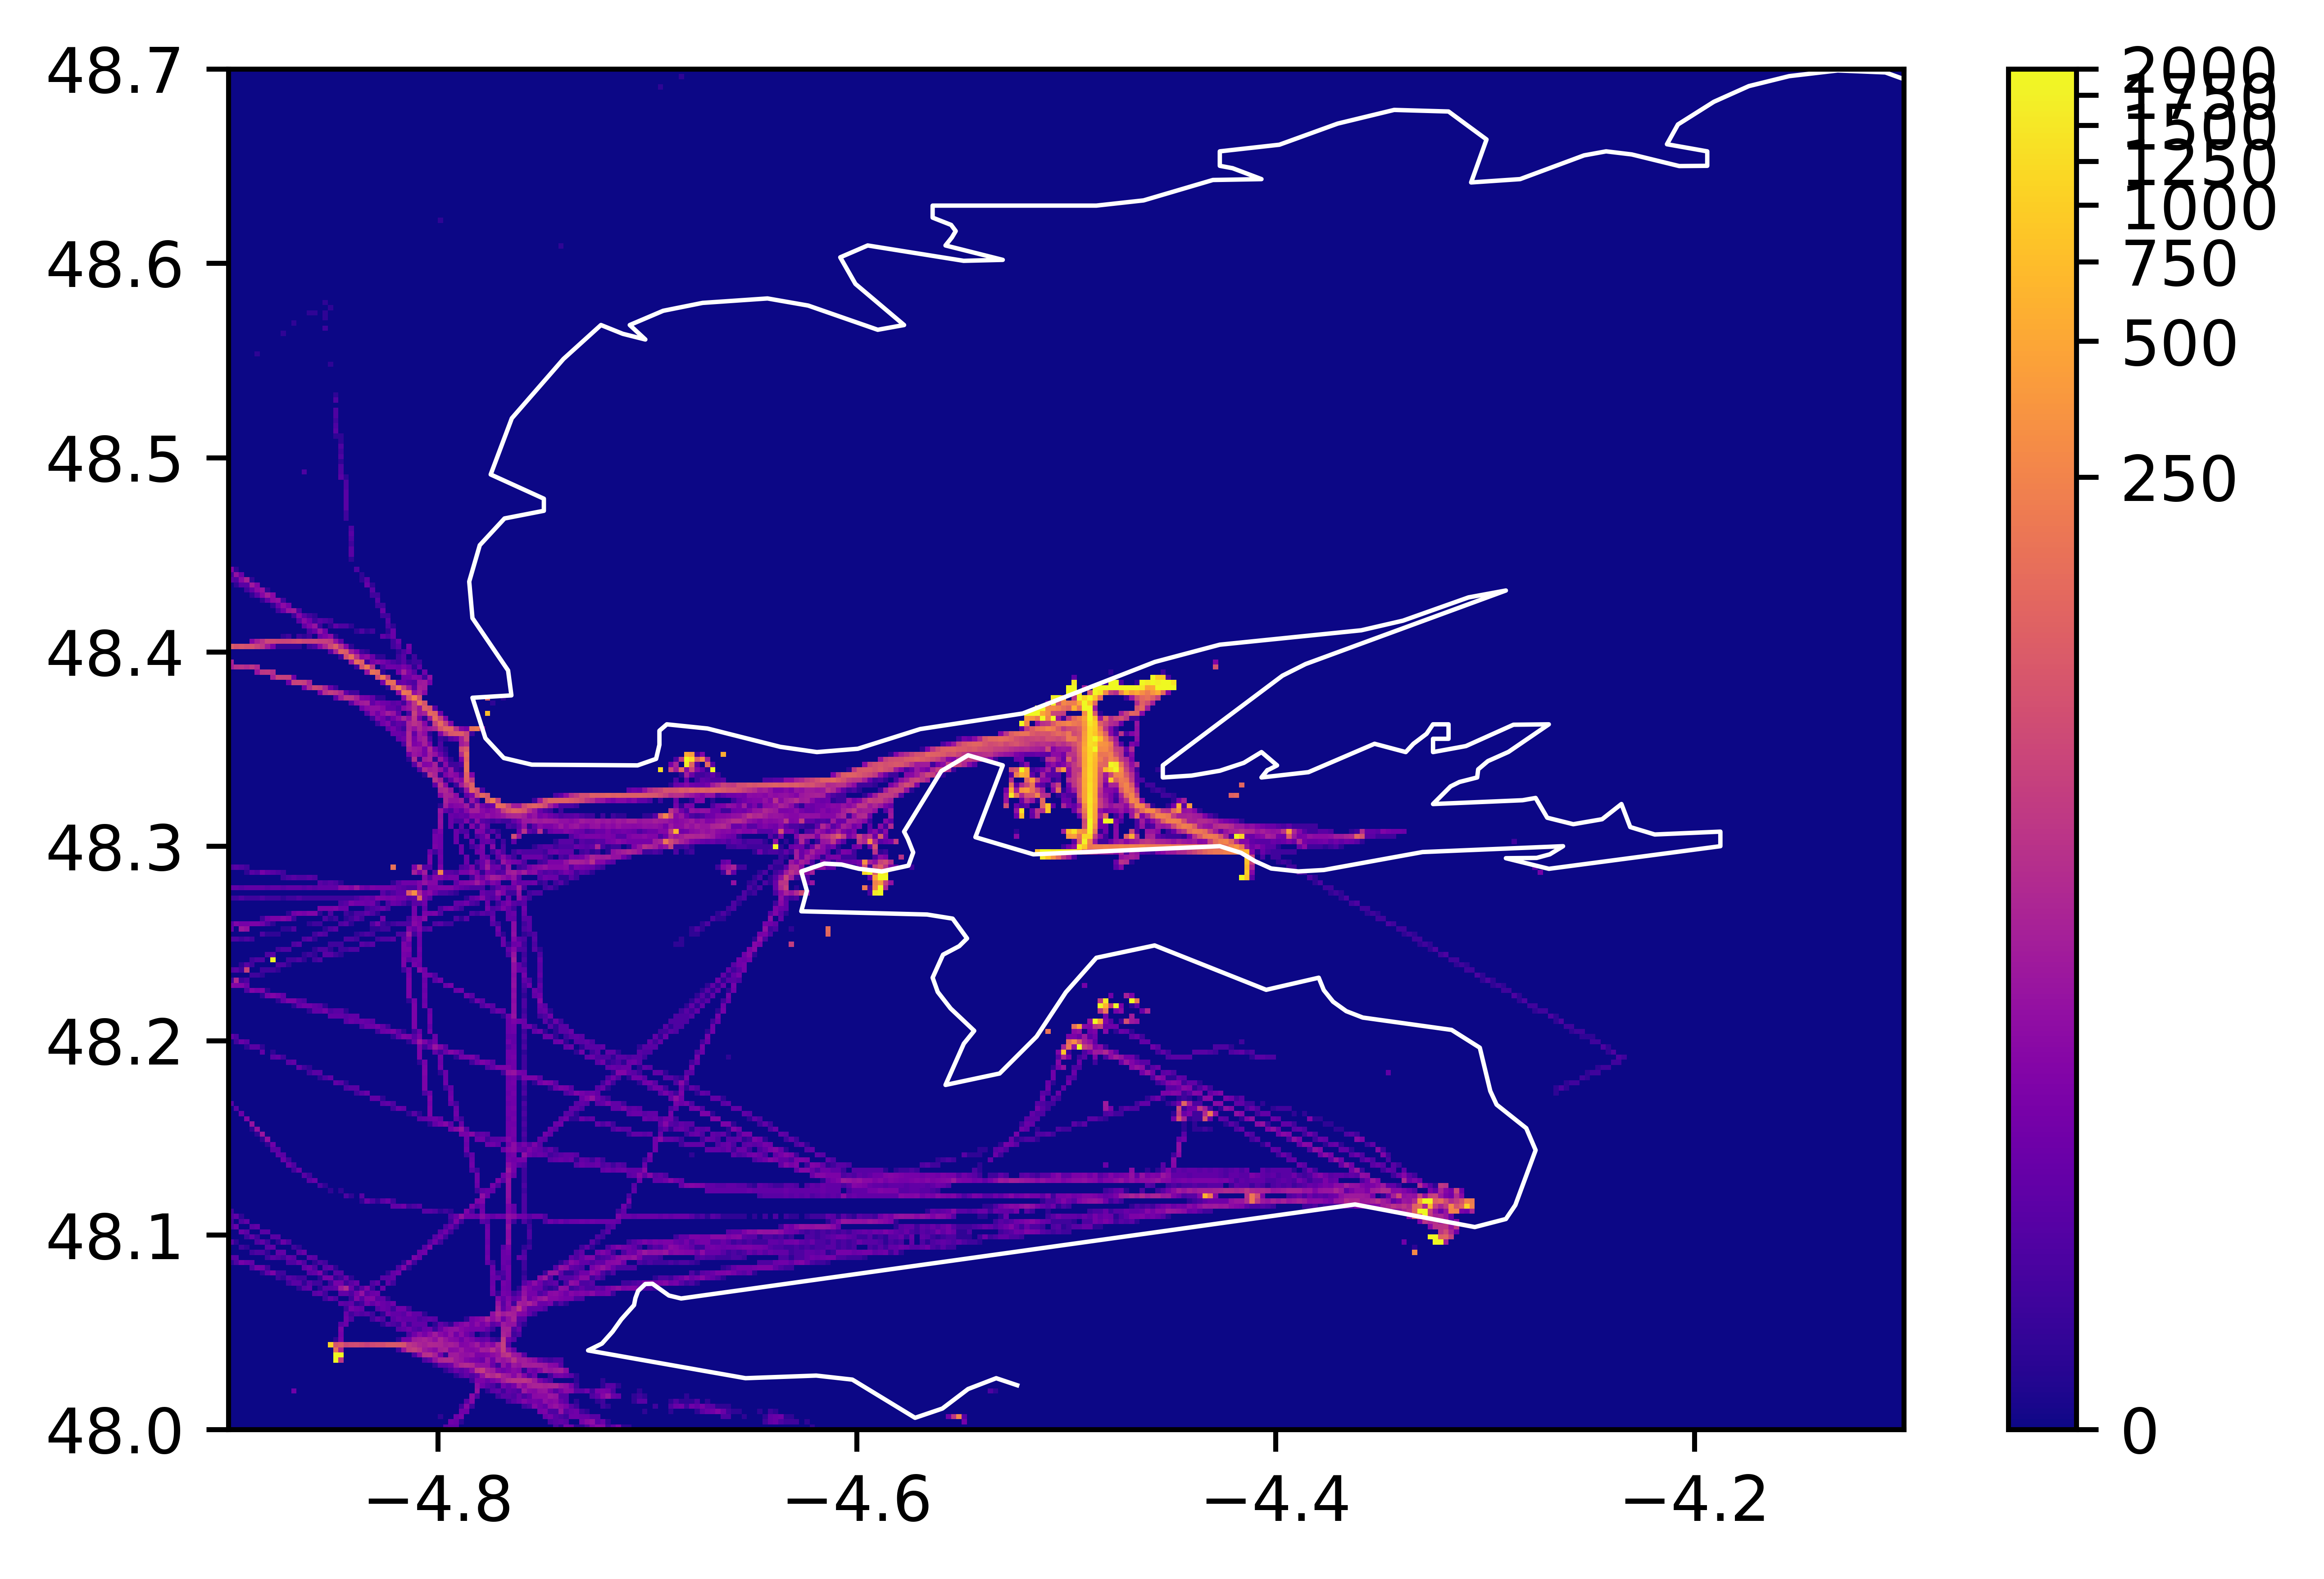
\includegraphics[scale=1]{figures/Ch5/ThesisExpStatusDensityZoom.png}
    \caption{Density map, with all the 5,5M occurrences of wrong Navigational Status, t}
    \label{fig: 5 Exp StatusDensityMap}
\end{figure}

What we were able to notice in Figure~\ref{fig: 5 Exp StatusDensityMap}, is that the high density areas where the Navigational Status is reported wrongly, are areas really close to port. As the AIS navigational status needs to be changed each time the vessel arrives at port. This led us to believe that the crew members "forgets" to change the navigational status, while in port. Which is then represented on the data, as the Vessel being stopped on port for long periods of time with the navigational status 0(under way using engine). This is we can see for the 

\subsection{ADS - Fishing Status Validation Experiment}

\section{Real Results Validation}






